\subsection{Property Graphen}
Property Graphen erweitern das Modell des einfachen Graphen.
Property Graphen sind gerichtete Graphen, die sich durch ihre den Kanten und Knoten zugewiesenen Eigenschaften (Properties) auszeichnen.
Gespeichert werden diese Eigenschaften als Key-Value-Paare.
Das Hinzufügen von Attributen an einen Knoten oder eine Kante soll zusammengehörige Daten schneller abrufbar machen \cite{angles2012comparison}.
Label ermöglichen die Unterteilung von Knoten und Kanten in verschiedene Knoten- und Kantentypen.
Attribute, Label und die Richtung der Kanten erlauben eine sehr detaillierte Modellierung von realen Sachverhalten.
Somit sind Property Graphen von sehr großer Bedeutung für die Modellierung von Graphdatenbanken.

Abbildung \ref{2.property.image} zeigt einen Property Graphen.
Die Knoten sind den drei Labeln Person, Unternehmen und Stadt zugeordnet.
Die gerichteten Kanten stellen die Beziehungsverhältnisse zwischen den einzelnen Knoten her und können durch Attribute, wie beispielsweise der Information über die Dauer der bisherigen Beziehung, genauer definiert werden.
\begin{figure}[H]
\begin{center}
	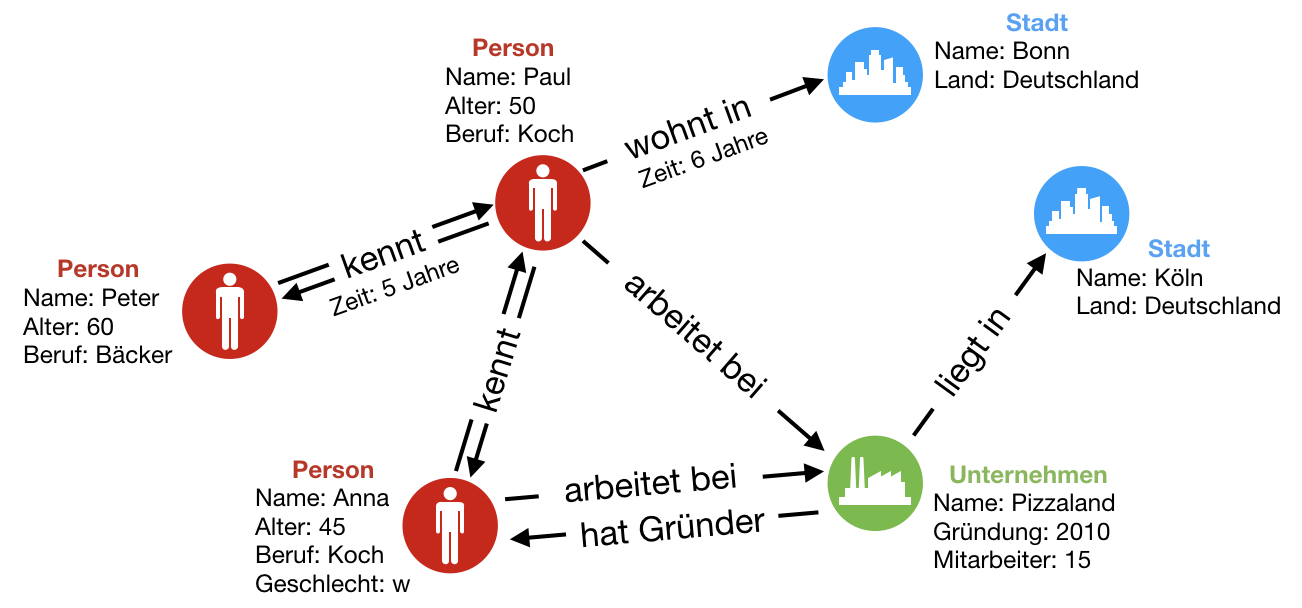
\includegraphics[scale = 0.65]{./images/Property_graph.png}
	\label{2.property.image}
	\caption{Property Graph}
\end{center}
\end{figure}


Der Vorteil von Property Graphen ist, dass diese eine sehr detailierte Modellierung der Daten ermöglichen.
Nachteilig ist, dass eine komplexere Datenstruktur zu einer komplizierteren Realisierung führt.
Derzeit sind Property Graphen das am häufigsten verwendete Datenmodell für Graphdatenbanken.
Neo4j, die momentan weltweit populärste Graphdatenbank, nutzt Property Graphen als Datenbankmodell \cite{neo4j}.
Ein weiteres Beispiel für ein Graph \ac{DBMS}, welches Property Graphen zur Modellierung nutzt, ist JanusGraph \cite{janus}.

\subsection{Hypergraphen}
Hypergraphen stellen eine Generalisierung von Graphen dar und ermöglichen die Modelierung komplexer Beziehungen \cite{anglesintro}.
%Hypergraphen haben die Eigenschaft, dass Kanten im Gegensatz zu klassischen Graphen mehr als zwei Knoten miteinander verbinden können.
%Die Kanten des Hypergraphen werden auch als Hyperkanten bezeichnet.
Im Vergleich zum normalen Graphen können die Kanten eines Hypergraphen eine beliebige Kardinalität haben.
Die Hyperedges in einem Hypergraphen verbinden somit eine beliebige Menge von Knoten, was eine direkte Darstellung von Beziehungen höherer Ordnung ermöglicht \cite{iordanov2010hypergraphdb}.
Im Falle eines gerichteten Hypergraphen verbindet die Hyperkante den Ausgangsknoten direkt mit allen Zielknoten.
%\\Mathematisch ist ein Hypergraph folgendermaßen definiert:
%\begin{definition}
%	Let $X=\{v_{1}, v_{2},...,v_{n}\}$ be a finite set,
%	and let $E=\{e_{1},e_{2},...,e_{m}\}$ be a family of subsets of $X$ such that
%	\[e_{i} \neq \varnothing (i=1,2,...,m) \\
%	\cup_{i=1}^{m}e_{i}=X.
%	\]
%	The pair $H=(X,E)$ is called a hypergraph with vertex set $X$
%	and hyperedge set $E$. The elements $v_{1}, v_{2},...,v_{n}$ of $X$ are vertices
%	of hypergraph $H$, and the sets $e_{1}, e_{2},...,e_{m}$ are hyperedges of hypergraph $H$ \cite[Seite 2]{zhang2018hypergraph}.
%\end{definition}

Abbildung \ref{2.hyper.image} zeigt einen Hypergraphen.
Die Kante $e_{4}$ verbindet in diesem Graphen die Knoten $v_{5}$, $v_{6}$ und $v_{7}$ miteinander.
\begin{figure}[H]
\begin{center}
	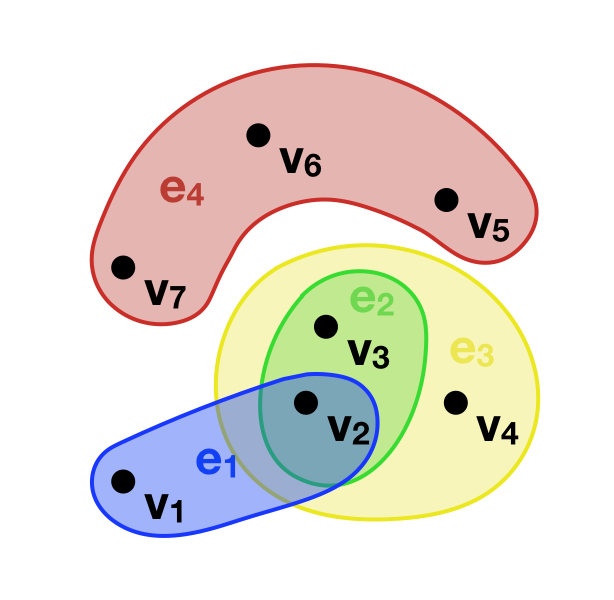
\includegraphics[scale = 0.5]{./images/Hypergraph2.png}
	\label{2.hyper.image}
	\caption{Hypergraph}
\end{center}
\end{figure}
%Hypergraphen ermöglichen die direkte Darstellung rekursiver Beziehungen \cite{iordanov2010hypergraphdb}.
Da Hypergraphen die direkte Darstellung rekursiver Beziehungen ermöglichen und somit eine flexiblere Struktur als das einfache Graphen-Modell bieten, werden diese oft zur Modellierung in Graphdatenbanken verwendet \cite{iordanov2010hypergraphdb}\cite{flockdb}.
Eine Datenbank, die Hypergraphen als Datenbankmodell nutzt ist beispielsweise HyperGraphDB, welche von Kobrix Software Inc entwickelt wurde \cite{iordanov2010hypergraphdb}.
Ein weiteres Projekt, bei dem Hypergraphen zur Modellierung genutzt werden ist Trinity \cite{shao2013trinity}.
%In einem normale Graphen sind die Kanten, eine in einem Intervall festgelegte Menge von Knoten:
%    \[X = \{v_{1}, v_{2}, v_{3}, v_{4}, v_{5}, v_{6}, v_{7}\} \text{ Knoten}\]
%    \[E=\{e_{1}, e_{2}, e_{3}, e_{4}\} \text{ Kanten}\]
%    \[E=\{e_{1}, e_{2}, e_{3}, e_{4}\} = \{\{v_{1}, v_{2}, v_{3}\}, \{v_{2}, v_{3}\}, \{v_{3}, v_{5}, v_{6}\}, \{v_{4}\}\} \]
%Transversals
%\subsection{Multimodale Graphen}
%\subsection{Hypertree}
%\subsection{k-uniform hypergraph}
\subsection{Verschachtelte Graphen}
%Hypernodes ermöglichen die Verschachtelung von Graphen, was bedeutet, dass ein Knoten wiederum ein Graph sein kann
In einem verschachtelten Graphen kann ein Knoten wiederum ein Graph sein. Diese Knoten werden als Hypernodes bezeichnet.
Das Konzept von Hypernodes erlaubt eine beliebig große Komplexität des Modells.
Das Hypernode Modell nutzt gerichtete Kanten.
Jeder Knoten des verschachtelten Graphen bekommt ein eindeutiges Label.
Um die Knoten in verschiedene Kategorien zu unterteilen werden Tags vergeben \cite{poulovassilis1994nested}.

Abbildung \ref{2.hypernode.image} stellt einen Teil des in \ref{2.property.image} dargestellten Property Graphen als Hypernodes dar.
Alle Knoten haben ein eindeutiges Label und es wurden zwei Tags vergeben - Unternehmen und Person.
Durch gerichtete Kanten werden die Beziehungen zwischen den einzelnen Hypernodes hergestellt.
Die Attributer, die im Property Graphen als Key-Value Paare gespeichert werden, werden im verschachtelten Graphen als Knoten einer Hypernode gespeichert.
\begin{figure}[H]
	\begin{center}
		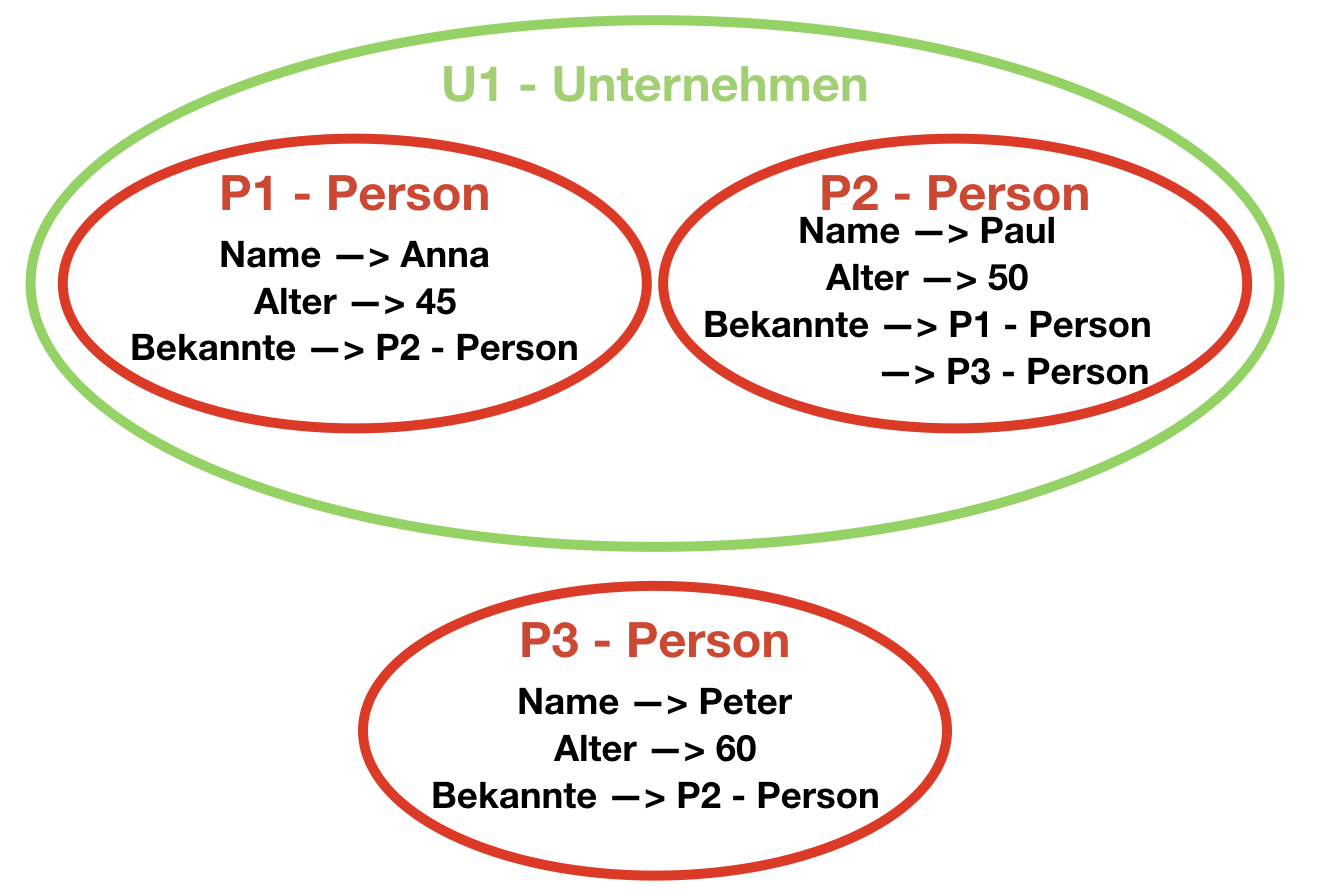
\includegraphics[scale = 0.5]{./images/Hypernode.png}
		\label{2.hypernode.image}
		\caption{Hypernode}
	\end{center}
\end{figure}

Hypergraphen lassen sich durch Hypernodes darstellen, indem man die im Hypergraph durch eine Hyperedge verbundenen Knoten in einer Hypernode modelliert.
Umgekehrt lassen sich Hypernodes nicht unbedingt in einem Hypergraphen realisieren \cite{poulovassilis1994nested}.